\documentclass[conference]{IEEEtran}
\usepackage{amsmath,epsfig}
\usepackage{graphicx}
\usepackage{epsfig,latexsym}
\usepackage{amsmath,amsfonts,amssymb,color}
\usepackage{graphicx}
\usepackage{subfigure}
\usepackage{multirow}
\usepackage{bbm}
\usepackage[T1]{fontenc}
\usepackage{url}
\renewcommand{\textfraction}{.01}
\renewcommand{\bottomfraction}{.99}
\renewcommand{\topfraction}{.99}

% correct bad hyphenation here
%\hyphenation{op-tical net-works semi-conduc-tor}


\begin{document}
%
% paper title
% can use linebreaks \\ within to get better formatting as desired
\title{Fireworks: Evolutionary Art Project based on EvoSpace-Interactive}


% author names and affiliations
% use a multiple column layout for up to three different
% affiliations

%\author{\IEEEauthorblockN{Michael Shell}
%\IEEEauthorblockA{School of Electrical and\\Computer Engineering\\
%Georgia Institute of Technology\\
%Atlanta, Georgia 30332--0250\\
%Email: http://www.michaelshell.org/contact.html}
%\and
%\IEEEauthorblockN{Homer Simpson}
%\IEEEauthorblockA{Twentieth Century Fox\\
%Springfield, USA\\
%Email: homer@thesimpsons.com}
%\and
%\IEEEauthorblockN{James Kirk\\ and Montgomery Scott}
%\IEEEauthorblockA{Starfleet Academy\\
%San Francisco, California 96678-2391\\
%Telephone: (800) 555--1212\\
%Fax: (888) 555--1212}}

% make the title area
\maketitle


\begin{abstract}
%\boldmath

\end{abstract}
% IEEEtran.cls defaults to using nonbold math in the Abstract.
% This preserves the distinction between vectors and scalars. However,
% if the conference you are submitting to favors bold math in the abstract,
% then you can use LaTeX's standard command \boldmath at the very start
% of the abstract to achieve this. Many IEEE journals/conferences frown on
% math in the abstract anyway.

% no keywords
\begin{IEEEkeywords}
Distributed algorithms, cloud computing, interactive evolutionary algorithm, linear genetic programming.
\end{IEEEkeywords}



% For peer review papers, you can put extra information on the cover
% page as needed:
% \ifCLASSOPTIONpeerreview
% \begin{center} \bfseries EDICS Category: 3-BBND \end{center}
% \fi
%
% For peerreview papers, this IEEEtran command inserts a page break and
% creates the second title. It will be ignored for other modes.
\IEEEpeerreviewmaketitle

\section{Introduction}
Artificial evolution has proven to be a powerful computational paradigm used to solve optimizaci�n, search and learning problems in diverse domains.
Moreover, evolutionary algorithms (EAs) have found a wider application area that traditional engineering or science, with promising contributions to art, music and
design being developed at a steady pace over recent years \cite{}. The nature of EAs, which combines a balanced mixture of
greedy optimization with explorative search, has allowed EAs to become robust and versatile algorithms that solve difficult
non-linear and discontinuos problems, even in cases where an analytic or automatic objective function cannot be derived \cite{}.

In particular, when dealing with creative domains, fitness usually needs to incorporate some sort of human knowledge and preferences,
either off-line (before the search) or on-line (during the search). The latter case refers to what are commonly known as interactive EAs (IEA).
Human interaction is required in these domains because creativity and aesthetic principles are not yet fully understood, which limits
the possibility of measuring them directly and objectively. That is why researchers have turned towards humans to provide an indirect and subjective
evaluation of evolved artistic artifacts.
While the IEA approach solves one problem, it also creates others, considering the following.
First, a human can easily get tired of what can be a monotonous task of evaluating many individuals over many generations (most of which will not be very interesting).
Secondly, a user can get bored, and start to provide feedback that deviates from the original goal of the system.
Finally, given the subjective nature of evaluating artistic design, a single user might not provide the required feedback; i.e. the fitness landscape might not
present the necessary structure for the search to proceed successfully.
Nonetheless, IEAs have been used to generate impressive artistic designs \cite{},
incorporating insights from computer science and artificial intelligence researchers, as well as artists from various domains.

Only until recently, however, has an EA tool been proposed that is specifically aimed at IEA
for artistic design.
EvoSpace-Interactive was developed with this goal in mind, providing a simplified development
interface for IEAs \cite{}.
Moreover, EvoSpace-Interactive was designed to incorporate and combine the subjective opinions from different users of the system.
Finally, EvoSpace-Interactive employs a cloud-based population manager that allows for asynchronous and distributed interaction from users, and employs social network integration to promote user collaboration and interaction.

In \cite{}, the EvoSpace tool is presented and in \cite{} a proof-of-concept implementation was presented for an IEA. In this work, on the other hand, a more advanced artistic IEA is
proposed, called \emph{Fireworks}.
Fireworks employs a linear genetic programming (LGP) approach to evolve artistic animations
of particle swarms that visually resemble a fireworks display.

The remainder of this paper proceeds as follows.
First, Section \ref{sec:related} presents a discussion of related works.
Then, Section \ref{sec:evo} presents the EvoSpace platform for IEAs.
The \emph{Fireworks} system is described in Section \ref{sec:fire}, detailing
the LGP algorithm and Processing based representation of individuals.
Experimental results are summarized and discussed in Section \ref{sec:exp}.
Finally, Section \ref{sec:conclude} outlines the main conclusions of this work.

\section{Related Work}
\label{sec:related}
The goal of IEAs is to use human preferences as the main (or only) source of selective
pressure that guides an evolutionary search \cite{ie1,ie2}.
IEAs pose an open-ended search where  the objective function used by traditional EAs is replaced by the subjective
preferences and interaction by a user of the system.
Indeed, some of the earliest EAs were open-ended systems, such as the well-known Biomorphs algorithm \cite{biomorphs}.
Therefore, IEAs should encourage high diversity and exploration given the dynamic and non-deterministic nature of the evaluation process,
such as in the novelty search based IEA proposed in \cite{ns:2012}.

IEAs have been used in various domains and applications;
for instance, \cite{} uses an IEA to evolve medical implants to improve a patients hearing.
However, this work focuses on the use of use interaction to evolve artistic artifacts using a collaborative and distributed approach.
IEAs that incorporate user collaboration and interaction are here referred to as collaborative IEAs or C-IEAs;
some noteworthy works in this area are reviewed next.

An early example of a web based interactive system is the work by Langdon \cite{langdon:2004}, where fractal representations of virtual creatures are evolved.
It proposed a distributed EA using a global population that resides on a central web server and uses Javascript to distribute
portions of the population to remote clients on the web.
Users evaluate individuals locally and those a user prefers are returned to the server and can be distributed again to others,
thus promoting a collaborative process during evolution.
Similarly, Secretan et al. \cite{picbreeder} and Clune and Lipson \cite{forms} use web-based IEAs to evolve artistic artifacts
using compositional pattern producing networks as a generative encoding.
In \cite{picbreeder} images are evolved, while 3-D sculptures are evolved in \cite{forms}.
In both cases, users (connected clients) are encouraged to collaborate.
In both works a central websites was developed where users can select or create random individuals and evolve lineages of artifacts based on their preferences.
In these systems a user can take a previously evolved artifact and continue the search process himself, building upon earlier design in a sequential
manner.
In this way, the evolved artifacts can be the product of a collaborative evolutionary search.
Another feature is that evolved artifacts can be rated by users, and given that users can create individual accounts, the ratings provide a way to rank users,
or to select previously evolved artifacts based on the particular style of each user.
Furthermore, the collaborative process is captured by the system, since it is possible to visualize how, and when, different users influenced
a genetic lineage.
Kowaliw et al. \cite{evoeco} present recent example based on evolving ecosystemic models, a generative encoding based on multi-agent systems
that generate high quality artistic drawings.
Again, users visit a website and interact with a Java applet,
after which they can choose to add evolved images to a central collection such that other users can see them or them as seeds for their own evolutionary design.


The present work builds on previous proposals and extends the C-IEA approach.
First, it promotes collaborative evaluations of artistic artifacts in a dynamic and parallel manner,
instead of the sequential approach followed in \cite{picbreeder,forms}.
Second, it incorporates explicit user interactions by encouraging the use of social networking.
Third, it facilitates the ability to save and share promising artifacts.
Finally, it emphasizes the use of a cloud-based model.

\section{EvoSpace}
\label{sec:evo}
EvoSpace is a population store for the development of evolutionary algorithms that are intended to run on a cloud computing model \cite{}.
It is designed to be versatile, since the population is decoupled from any particular evolutionary algorithm.
Evospace is asynchronous, client processes, called EvoWorkers, dynamically and asynchronously interact with the EvoSpace store and perform the basic
routines of an evolutionary search.
EvoWorkers can reside on remote clients or on the platform server itself.
The EvoSpace platform is presented in \cite{}, here we only provide a general outline of how the system functions.

EvoSpace consists of two main components.
The first component is the EvoSpace container, used to store the population of an EA.
The second component consists of the remote clients or EvoWorkers, which
execute the actual evolutionary process.
Figure \ref{fig:evo} presents a block schematic diagram of the EvoSpace system and data flow.

\begin{figure*}[t]
    \centering
        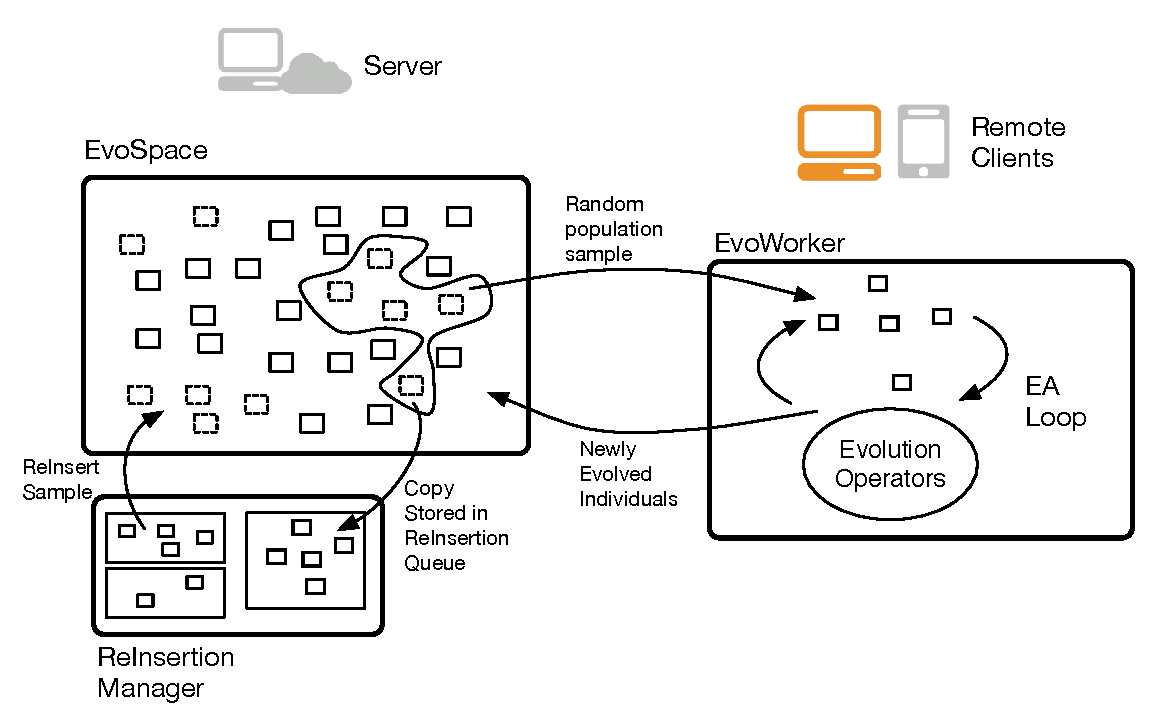
\includegraphics[width=14cm]{evospaceExample.eps}
    \caption{Main components and dataflow within EvoSpace.}
    \label{fig:evo}
\end{figure*}



\subsection{The EvoSpace container.}
EvoSpace is based on the tuplespace model, a distributed shared memory (DSM) abstraction, organized as a \emph{bag} of tuples.
A tuple $t$ is the basic tuplespace element, composed by one or more fields and corresponding values.
In this model, the basic operations that a process can perform is to insert or withdraw tuples from the tuplespace.
EvoSpace is composed by a set of objects $ES$ and a set of interface methods provided by a central server.
Objects can be withdrawn, processed and replaced into $ES$ using a specified set of methods.
%%, while also protecting access rights.
%However, EvoSpace is different from other tuplespace implementations in the sense that retrieving and reading objects from ES are random operations.
%Individual objects are not of high interest when accessing $ES$, neither is retrieving objects based on search criteria.
The current EvoSpace implementation offers the following interface methods.

\textbf{Read(n):} This method returns a random set $A$ of objects from $ES$, with $|A|=n$ and $A\subset ES$, if $n< |ES|$, the method returns $ES$ otherwise.

\textbf{Take(n):} Returns a random set $A$, following the similar logic used for $Read()$.
However, in this case the sequence of $Take()$ operations provide a temporal dimension to the dynamics of set $ES$.
We can define $ES_i$ as the set at the moment of the $i-th$ $Take()$ operation and $A_i$ as the output.
The contents of EvoSapce are then given by $ES_{i+1}= ES_i \setminus A_i$; i.e., the objets taken are effectively removed from $ES$.
The objects taken are also copied to a new set $S_i$ of \emph{sampled objects} and stored
within a temporary collection $\mathcal{S}$ on the server, implemented as a priority queue.
Sets $S_i \in \mathcal{S}$ can then be reinserted to $ES$ if necessary.

\textbf{ReInsert(i):} This method is used to reinsert the subset of elements removed by the $i-th$ $Take()$ operation,
  such that the contents of EvoSpace are now $ES \cup S_i$ if $S_i \in \mathcal{S}$ and $ES$ is left unchanged otherwise.

\textbf{Insert(A):} This method represents the union operation $ES \cup A$.

\textbf{Replace(A,i):} Similar to $Add()$, however set $A$ should be understood as a replacement for
  some $S_i \in \mathcal{S}$, hence $|A| = |S_i|$, but the objects in $A$ can be different (evolved) objects from those in $S_i$.
  Moreover, if $S_i$ exists it is removed from $\mathcal{S}$.
  However, if $S_i$ does not exist this means that a $ReInsert(i)$ operation preceded it, this increases the size of $ES$.

\textbf{Remove(A):} This method removes all of the objects in $A$ that are also in $ES$, in such a way that
  the contents of EvoSpace are now set to $ES \cup (A\cap ES)$.

The sub-components of EvoSpace are summarized below.

\emph{Individuals.}
The objects contained within $ES$ represent the evolving individuals of an EA.
Individuals in $ES$ are stored as \emph{dictionaries}, a collection of unique keys and values with a one to one association.


\emph{The EvoSpace Server.}
On the server side the \texttt{EvoSpaceServer} process creates and activates a new EvoSpace
container object and waits for requests to execute interface methods.
Three other server processes are also executed: \texttt{InitPopulation}, \texttt{ReInsertionMgr} and \texttt{EvolutionMgr}.
\texttt{InitPopulation} initializes the population with a total of $popsize$ random individuals.
\texttt{ReInsertionMgr} periodically checks (every $wt$ seconds) if the size of the population in $ES$
falls below a certain threshold $min$ or if the time after the last reinsetion is greater than $next_r$.
If any of these conditions are satisfied, then $rn$ subsets $S_i \in \mathcal{S}$ are reinserted into ES using the $ReInsertOld()$ method.
Finally, \texttt{EvolutionMgr} periodically checks if a termination condition is satisfied according to the needs of the evolutionary search.
For an open-ended IEA a termination criteria is usually not implemented, and is left up to the researcher to halt evolution when he sees pertinent.



\emph{EvoWorkers.}
The \texttt{EvoWorker} process requests a set of $ew_{take}$ individuals from the $ES$ container using the $Take()$ interface method provided by EvoSpace.
In the case of an IEA, the individuals are presented to a user of the system which is prompted to evaluate them.


\emph{Evolve Process.}
Finally, in the case of an IEA, after a pre-specified number of $Take()$ operations $evolve_{threshold}$ the $Evolve()$ function is invoked on the server side,
which proceeds to request a set of $ev_{take}$ individuals using the $Take()$ method, on which the specified set of genetic operators (selection, mutation, crossover, etc.)
are applied to generate new individuals or offspring which are then returned and reinserted into the population store.

\emph{Implementation of the population store.}
Individuals are stored in-memory, using the Redis key-value database.
Redis was chosen over a SQL-based management system, or other non-SQL alternatives, because it provides a hash based implementation of sets and queues which are natural data structures for the EvoSpace model. For example, selecting a random key from a set has a complexity of O(1). The logic of EvoSpace is implemented as a Python module exposed as a Web Service using cherrypy and Django HTTP frameworks. The EvoSpace web service can interact with any language supporting json-rpc or ajax requests. The EvoSpace modules and workers in JavaScript, JQuery and python are available with a Simplified BSD License from \url{http://evospace.org}.

\subsection{EvoSpace-Interactive.}
This paper presents a C-IEA system based on an extension of the EvoSpace platform called EvoSpace-Interactive \cite{},
depicted in a block diagram in Figure \ref{fig:CIE}.
With  EvoSpace-Interactive developers can exploit a platform for distributed user collaboration and interactive evolution,
that offers a central repository for the population implemented as an EvoSpace service;
a Web Application script implemented using Django, a mature full stack Web Framework with a BSD license developed in Python.
EvoSpace-Interactive is responsible for user authentication and session handling through the popular Facebook social network using the OAuth 2.0 protocol.
Also, the storage of collections, where users can store individuals they like to share with friends, is persisted using the PostgreSQL DBMS.
Most of the interactive functionality is programmed in the client side using Javascript libraries.
The communication between components is implemented using json-rpc, a lightweight remote procedure call protocol and common ajax and http transactions.
Overall functionality is decomposed in specialized services, adding flexibility to the framework since services can be interchanged.
The framework is build using only open source components from libraries to servers.
Users interact with the system through a GUI implemented on a Responsive Web Design (RWD) front end framework,
an approach to web design in which a graphical user interface is crafted to provide a satisfactory  viewing experience in a range of mobile devices.
This approach will enable designers to tailor the look and feel of the application with minimum intrusion, only changing CSS definitions.

Three components must be specified by the application developer, marked with double lines in Figure \ref{fig:CIE}; these are:
an \emph{individual} representation; a \emph{processing script} that renders each individual;
and a \emph{worker} script that encodes the evolutionary operators depending upon the proposed representation.

\begin{figure*}[t]
    \centering
        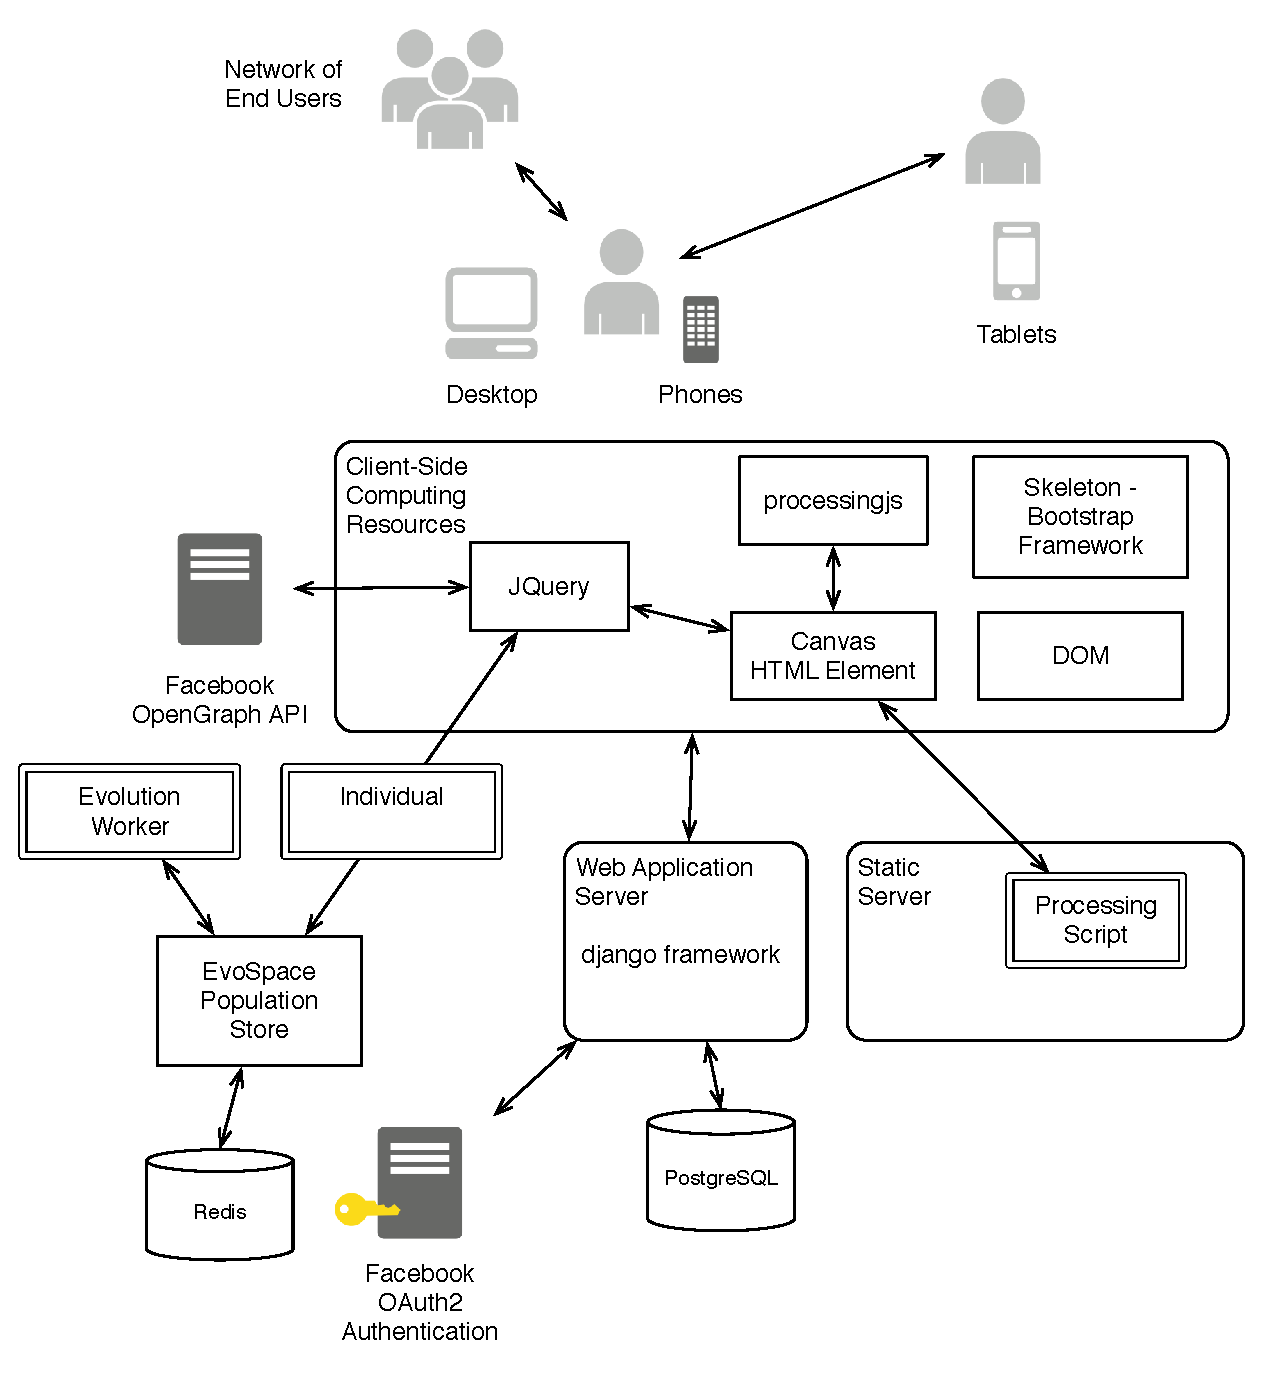
\includegraphics[width=14cm]{arq.eps}
    \caption{Conceptual design of the proposed C-IEA.}
    \label{fig:CIE}
\end{figure*}




\subsection{User Interface}
The users interact with the web interface composed of five elements proposed in \cite{}, depicted in Figure \ref{fig:web}.
First, at the top left corner user login, where users can link to their Facebook account or decide to participate as an anonymous user.
Second, to encourage user interaction when a user chooses to login to his Facebook account a list of friends that have also linked to the C-IEA application is presented
on the left.

\begin{figure}[t]
    \centering
        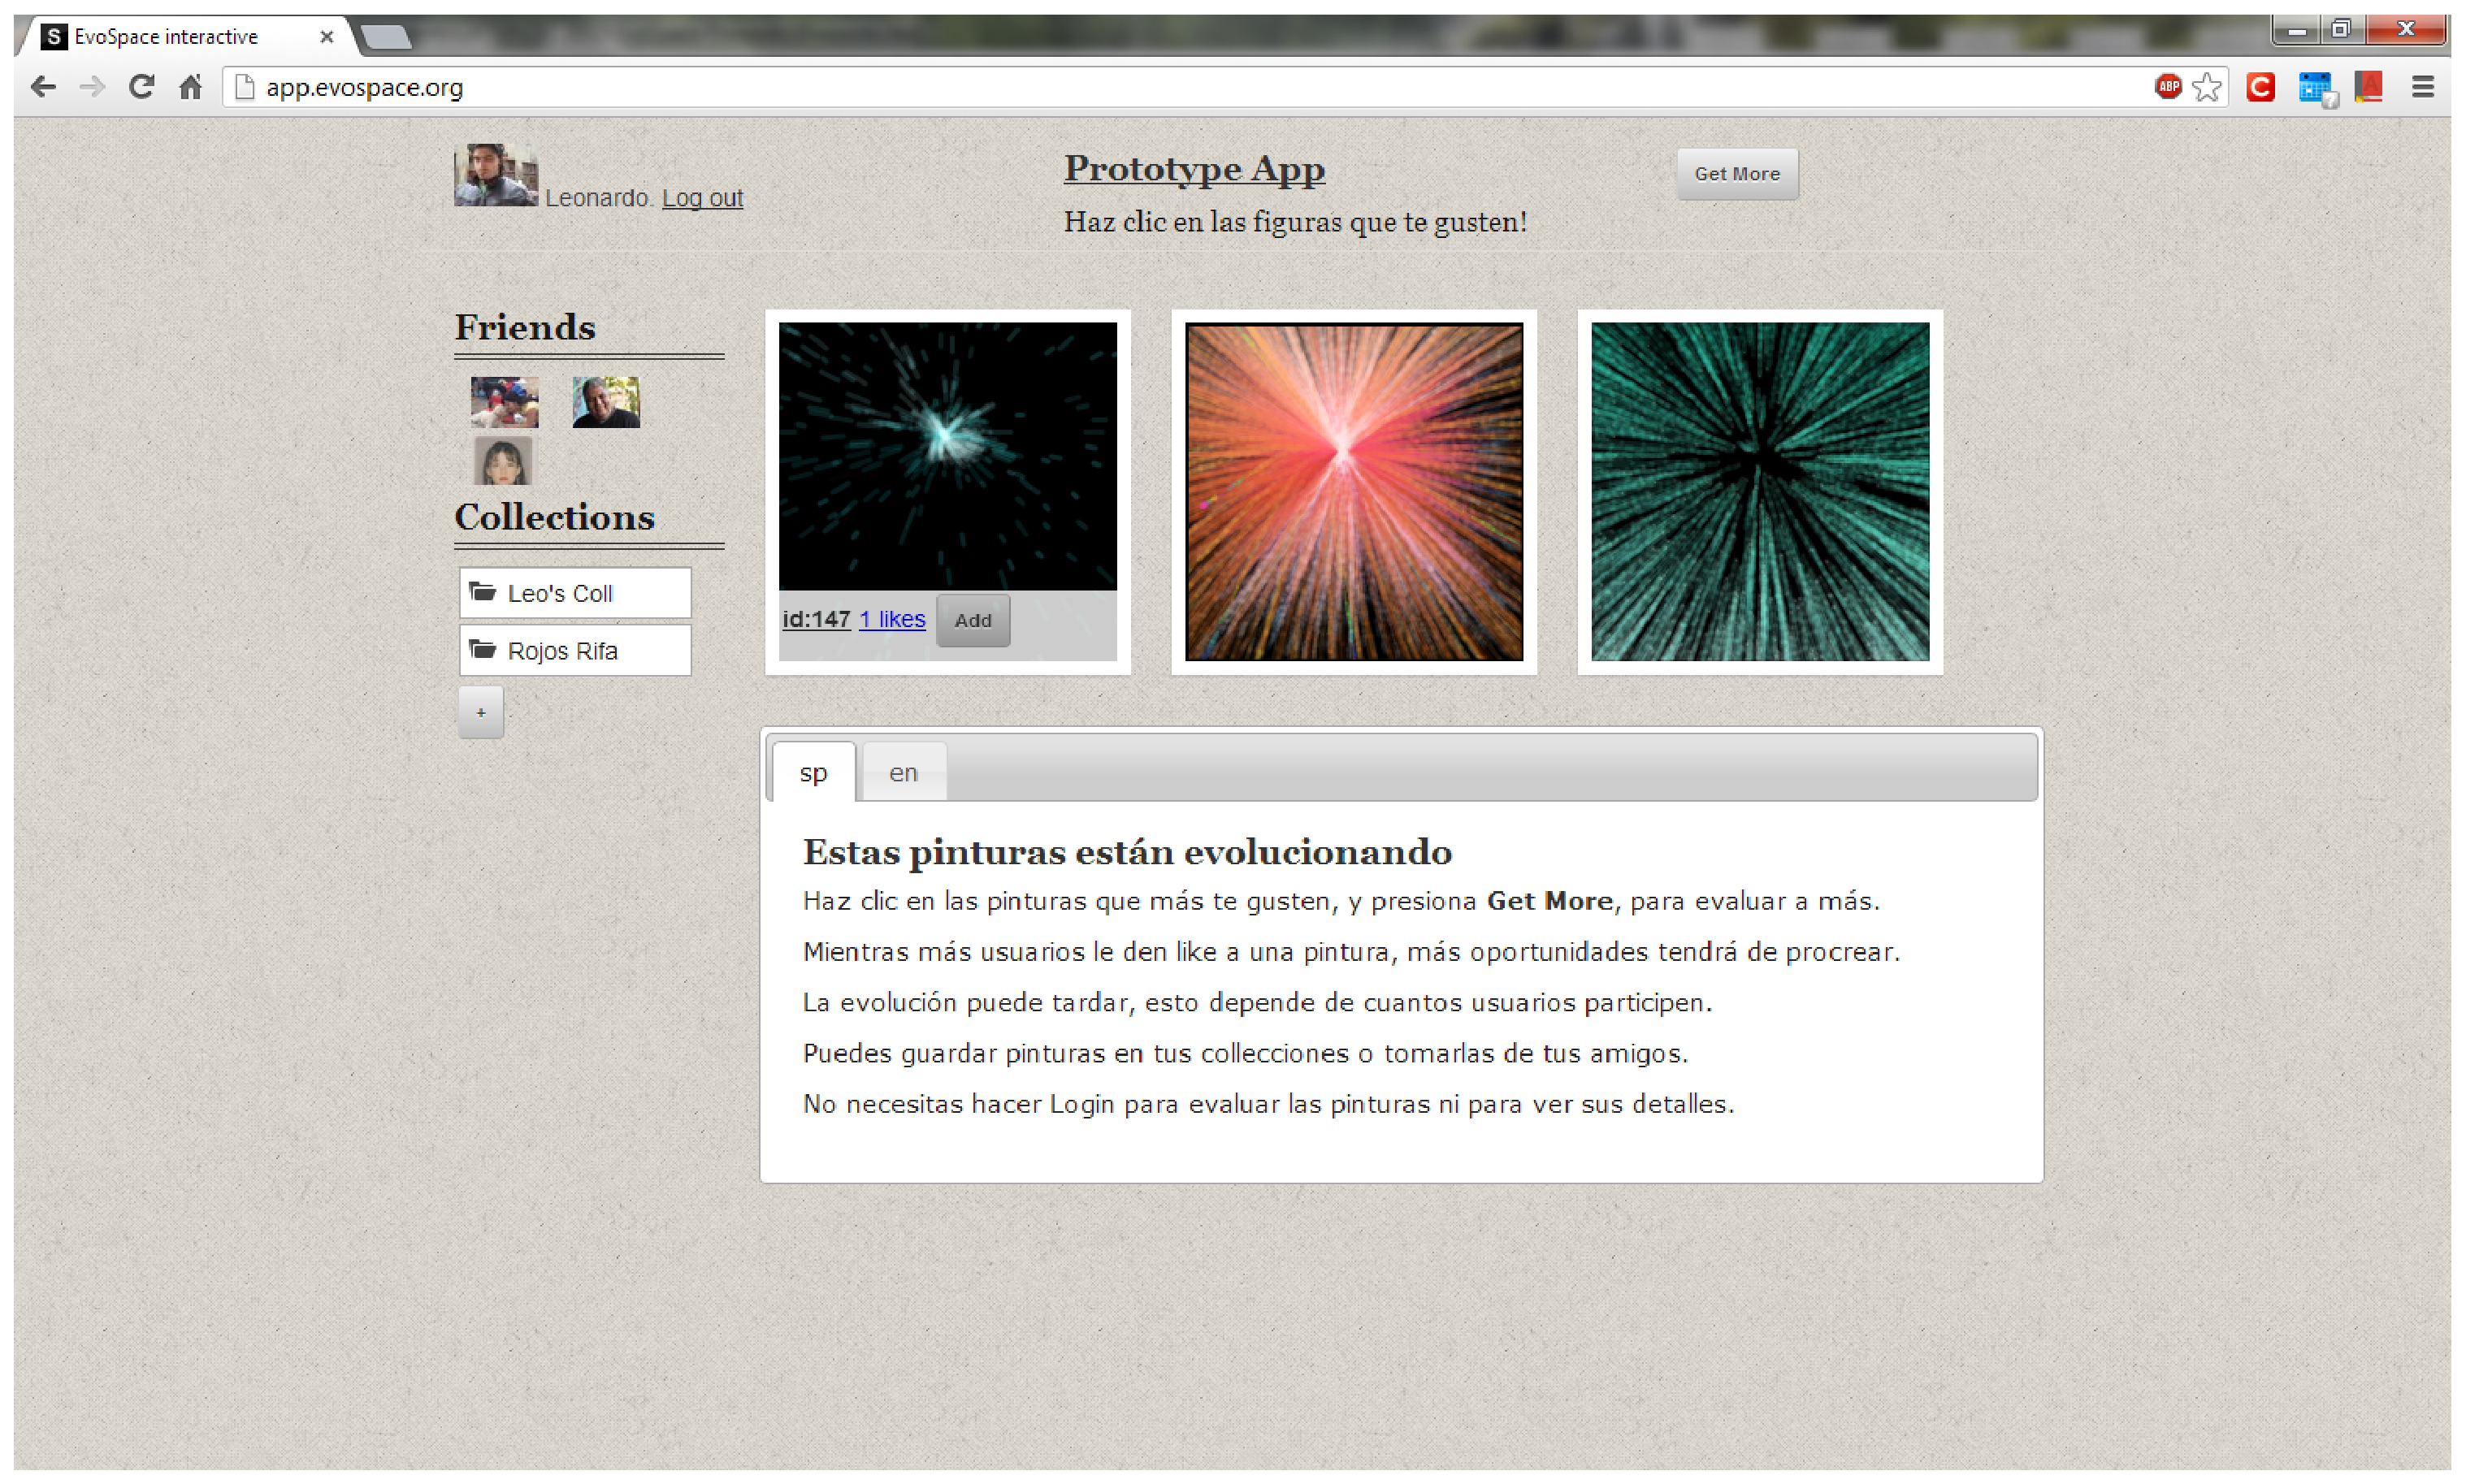
\includegraphics[width=8cm]{EvoApp.eps}
    \caption{User interface of the EvoApp C-IEA.}
    \label{fig:web}
\end{figure}

The third element is a central \emph{Wall} area, where $ew_{take}$ randomly sampled individuals by a $Take()$ operation are shown to the user..
Here, the user can interact with the system by clicking on the individuals he prefers, chich counts as a ''like" for the individual,
or the user can add an image to a \emph{collection} of individuals, a special directory to store individuals a user prefers and wishes to save.

After the user finishes interacting with the current crop of individuals he can choose to retrieve a new sample from EvoSpace.
This is done with the fourth element of the interface, located at the top of the screen, the \emph{GetMore} button.
The button returns the current group of individuals to EvoSpace, and brings back a new one.

The \emph{collections} section is the fifth element of the interface, shown at the bottom left corner.
The user can create as many collections as he wants to organized his preferred individuals.
Moreover, a user can browse the content of each collection and from there share images through the social network.
When a user browses over an individual a detail pane shows how many users have liked the individual.

\subsection{Individual Representation}
As stated above, individuals are represented internally as a dictionary.
The properties stored by EvoSapce-Interactive applications are: a unique \texttt{id}; a user defined \texttt{chromosome};
the number of times the individual has been selected in a sample and returned to the population, stored in property called \texttt{views};
the genetic operators that generated the individual; ids of the parents; \texttt{current Fitness} that stores the most resent fitness value;
and a \texttt{fitness} dictionary where each key is a concatenation of a \texttt{userid}, a \texttt{timestamp} and a numerical value that represents
the rating given by the corresponding individual.
A UML representation of an individual is presented in Figure \ref{fig:individual}.


\begin{figure}[t]
    \centering
        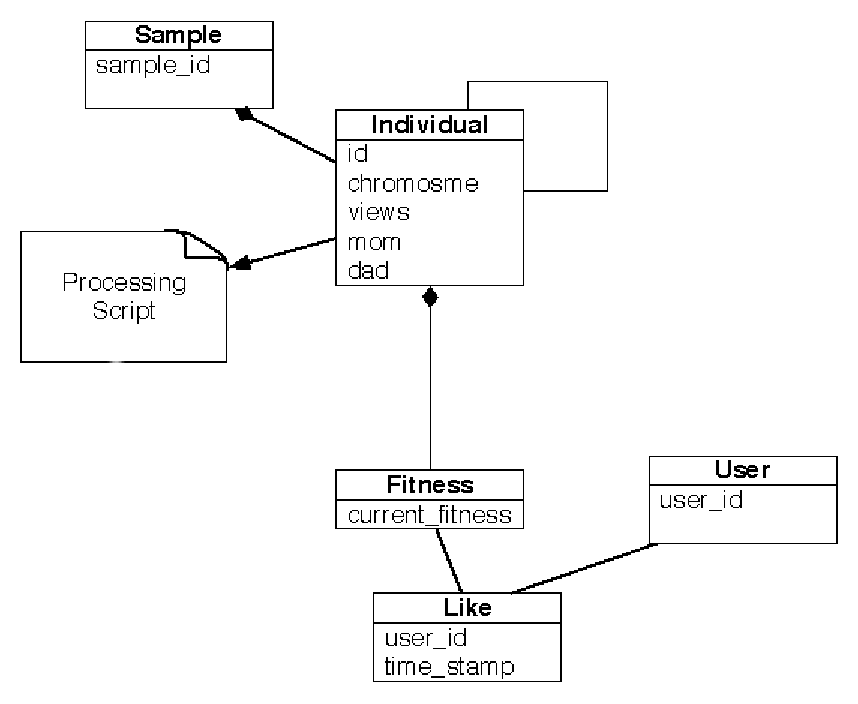
\includegraphics[width=8cm]{UMLIndividual.eps}
    \caption{Individual internal representation.}
    \label{fig:individual}
\end{figure}

\subsection{Processing Language and HTML Canvas Element}
Processing is a programming language and development environment initially created to serve as a software sketchbook and as a tool to teach fundamentals
of computer programming within a visual context.
Currently is used by artists, designers, architects, and researchers for visualization applications, games and interactive animations projects \cite{Reas:2007wp}.
Processing is a subset of Java directed to novice programmers and generative artists \cite{Pearson:2011ti}, which are the intended users of the EvoSpace-Interactive framework.
As a complement there is a javascript library \emph{processingjs} that allows Processing scripts to be run by any HTML5 compatible browser.
Processing scripts are responsible of rendering individuals which can involve animations, sound or even interactive artifacts.
Before calling the \texttt{draw()} method of the processing script initial place holding or fallback parameters are replaced with an individual's chromosome.
Each individual's script has its own Canvas entity, defined by the HTML5 standard as an element that provides scripts with a resolution-dependent bitmap canvas
which can be used for rendering graphics on the fly.
Although the combination of an HTML5 Canvas element and a Processing script is supported by default, other combinations could be used.
For instance, images, embedded audio, or other libraries capable of drawing in the Canvas.
Also, a fallback implementation must be considered for applications intended for non-HTML5 capable browsers.


\bibliographystyle{IEEEtran}
\begin{flushleft}
\bibliography{biblio}
\end{flushleft}



% that's all folks
\end{document}


